\subsubsection{Descripci\'on} 

\textbf{
K. Bertet [Bertet 2010] proposed the so called direct-optimal basis.
K. Adaricheva [Adaricheva 2012] proposed the so called D-basis as a subset of direct-optimal basis.
Open problem: Improving the computation of these basis (or something similar) to reduce massive closures computations in a second stage.}


\textbf{Direct-optimal basis computation by means of the fusion of Simplification rules, E. Rodr ́ıguez-Lorenzo et.al., Last review Discrete Appl. Math (2017)}

Una vez que hemos conseguido un algoritmo para el c\'alculo del cierre eficiente y optimizado, el siguiente paso para reducir el coste del c\'alculo del cierre es optimizar todo lo posible el sistema implicacional de entrada. Es aqu\'i donde entran en juego nuevos conceptos como son por ejemplo el de base directa \'optima. A continuac\'on se van a detallar algunos de estos conceptos.

\textbf{Base}

Un sistema implicacional \( \Sigma \) se dice que es:
\begin{itemize}
    \item una base minimal cuando,  \( para \ todo \ A \to B \in \Sigma \ se \ tiene \ que \ \Sigma \setminus \{A \to B\} \not\equiv \Sigma\)

    \item una base m\'inima cuando,  \( para \ todo \ \Sigma' \equiv \Sigma \ se \ tiene \ que \ |\Sigma| \leq |\Sigma'|\)

    \item una base \'optima cuando,  \( para \ todo \ \Sigma' \equiv \Sigma \ se \ tiene \ que \ \|\Sigma\| \leq \|\Sigma'\| \\ donde \ \|\Sigma\| = 
    \sum_{\substack{A \to B \in \Sigma}} (|A|+|B|) \).
\end{itemize}

\textbf{Directo}

Un sistema implicacional \( \Sigma \) se dice que es directo  cuando, \( para \ todo \ X \subseteq S \ se \ tiene \ que \\ X^+_{\Sigma} =  X \cup \bigcup\{ B | A \to B \in \Sigma \ para \ algun \ A \subseteq X \} \). Esto se traduce en que se puede calcular el cierre de un conjunto de atributos con una sola pasada y que ninguna de las implicaciones puede ser eliminada sin perder esta propiedad.

Por tanto, ya se esta en condiciones de conocer que es una base directa \'optima.
\newpage
\subsubsection{C\'odigo} 
\lstinputlisting{r_code/DO_IS.R}
\newpage
\subsubsection{Ejemplo} 
A continuaci\'on, se muestra un ejemplo del c\'alculo de una base directa optima a partir del siguiente conjunto de implicaciones: 
\begin{figure}[H]
    \centering
    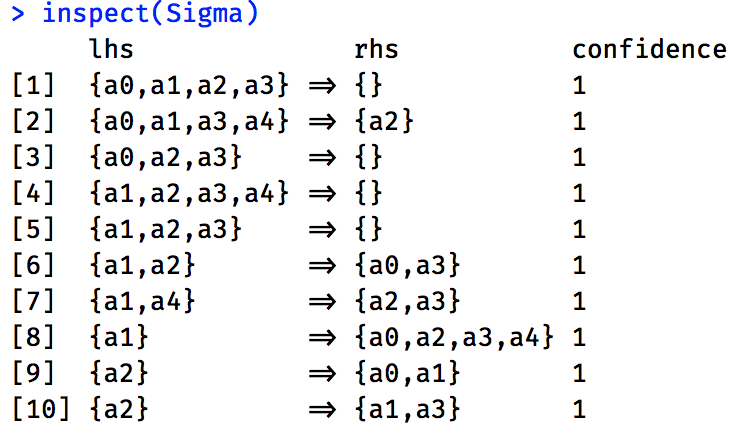
\includegraphics[scale=0.75]{do_1}
    \caption{Ejemplo SLgetDO 1}
    \label{fig:do_1}
\end{figure} 

Aqu\'i se puede ver el resultado:
\begin{figure}[H]
    \centering
    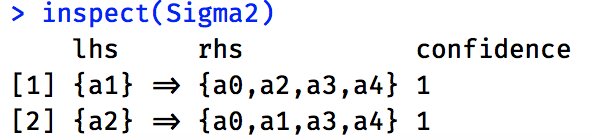
\includegraphics[scale=0.75]{do_2}
    \caption{Ejemplo SLgetDO 2}
    \label{fig:do_2}
\end{figure} 
Y, como era de esperar, el hecho de usar una base directa optima para el c\'alculo del cierre reduce consideradamente los tiempos de ejecuci\'on incluso en ejemplos tan peque\~nos como este, d\'onde el c\'alculo es practicamente inmediato.
\begin{figure}[H]
    \centering
    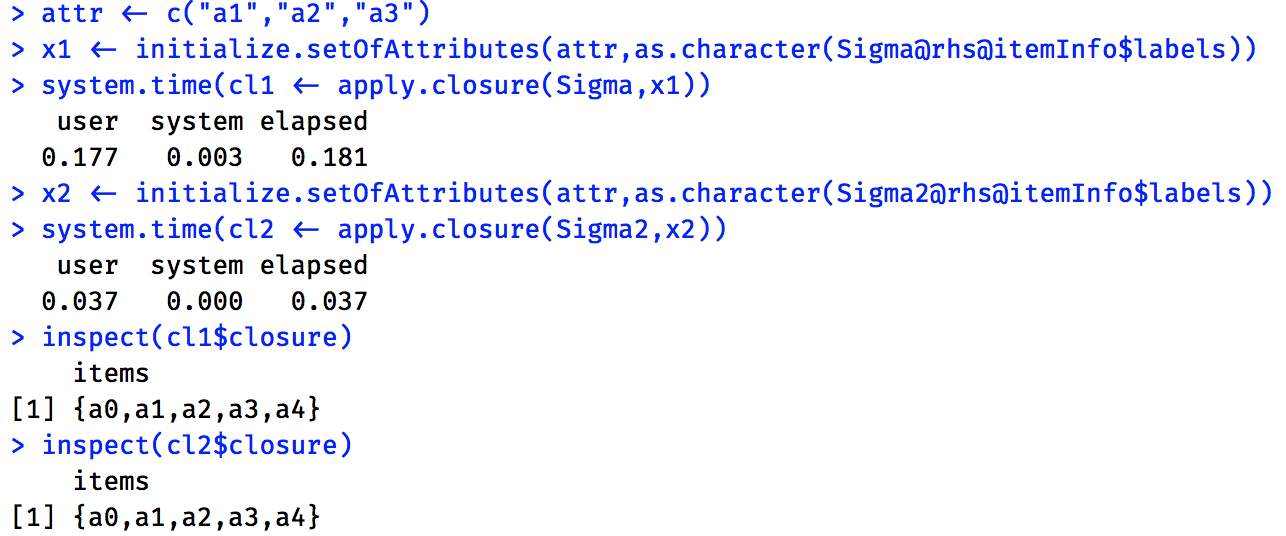
\includegraphics[scale=0.75]{do_3}
    \caption{Comparativa del c\'alculo del cierre a partir de una base DO}
    \label{fig:do_3}
\end{figure} 

Esta reducci\'on de tiempo se acent\'ua conforme crece el tama\~no del conjunto de implicaciones.

Si se tiene en cuenta que para resolver determinados problemas, el c\'calculo de multitud de cierres (del orden de millones) es parte fundamental,(REFERENCIA A DIRICHEVA) el impacto de cualquier peque\~na mejora en el c\'alculo de cada uno de esos cierres, puede suponer una diferencia abismal. De ah\'i radica la importancia de este algoritmo.
(¿ES EL PRIMERO?)
\subsubsection{Comparativa/Versiones} 